\documentclass[conference, twoside]{IEEEtran}

\usepackage{tikz}
\newcommand{\onethird}{2.333333333cm}

\usetikzlibrary{positioning,fit,matrix}
\tikzstyle{architecture_node_nofill}=[rectangle, draw, minimum height=1cm,anchor=north west]
\tikzstyle{architecture_node_fullwidth}=[architecture_node_nofill,minimum width=7cm]
\tikzstyle{architecture_box}=[draw=black,dashed,anchor=north west]
\tikzstyle{architecture_no_fill}=[fill=none] % To disable all fills
\usetikzlibrary{calc}

\definecolor{lightred}{HTML}{EA2424}
\definecolor{red}{HTML}{D0021B}
\definecolor{lightblue}{HTML}{7D9FC7}
\definecolor{blue}{HTML}{4A90E2}
\definecolor{purple}{HTML}{7571A1}
\definecolor{green}{HTML}{70A500}
\definecolor{lightgreen}{HTML}{C1FF7D}
\definecolor{lightyellow}{HTML}{F8E71C}
\definecolor{yellow}{HTML}{F5A623}
\definecolor{lightorange}{HTML}{F56023}
\definecolor{orange}{HTML}{EB4400}
\definecolor{waterblue}{HTML}{6BE4C9}


\usepackage{cite}

\usepackage{amsmath}
\usepackage[colorlinks]{hyperref}
\hypersetup{citecolor=black}
\hypersetup{linkcolor=black}
\hypersetup{urlcolor=black}
\usepackage{cleveref}
\usepackage{fancyvrb}

% format citations
\renewcommand\citepunct{, }
\renewcommand\citeleft{[}
\renewcommand\citeright{]}
\renewcommand\citedash{--}


\begin{document}
    % TITLE & PUBLICATION ID

    \title{An effective approach to defect detection} %  on steel surfaces
    \IEEEpubid{0000--0000/00\$00.00 ̃\copyright ̃2019 IEEE }

    % AUTHORS

    \author{
        \IEEEauthorblockN{Antonio Terpin}
        \IEEEauthorblockA{Electronic Engineering, Scuola Superiore\\
        Università degli Studi di Udine\\
        Udine, Italia \\
        Email: terpin.antonio@spes.uniud.it}
        \and
        \IEEEauthorblockN{Claudio Verardo}
        \IEEEauthorblockA{Electronic Engineering, Scuola Superiore\\
        Università degli Studi di Udine\\
        Udine, Italia \\
        Email: verardo.claudio@spes.uniud.it}
    }

    \maketitle

    \begin{abstract}
    Quality control is a main issue in any industry. The need of assuring a human-like evaluation during products quality control has resulted in an active research aiming to develop an automatic defect detection scheme.
    In this paper an effective solution to defect detection on steel surfaces from images is presented. Firstly, a preprocessing step aiming to spot plausible defective areas is discussed. Lastly, the classification of these proposed regions is made. Hence, a proper segmentation scheme is described. Incidentally, a novel usage of the dilation factor in convolutional layers is introduced, providing an effective approach to classifying images of different sizes.
\end{abstract}

\begin{IEEEkeywords}
    Defect Detection, Computer Vision, Deep Learning, Wavelet.
\end{IEEEkeywords}
    \section{Introduction}
    \par{
        A fundamental aim in any industry is to design highly efficient and effective quality control processes. Therefore, the research area focusing on automatic defect detection systems has become even more fecund in the last decades. 
    }
    \par{
        There is a large variety of previous work on defect detection on steel surfaces \cite{ieee:4777721, ieee:7030439, ieee:8623728, ieee:1334512, ieee:6738559}. Many ideas \cite{ieee:4777721, ieee:7030439, ieee:8623728} bank on the uniformity of the background surface, while other solutions use deep learning architectures \cite{ieee:1334512, ieee:6738559}, which provide an attempt to a robust defect segmentation. More refined approaches rely on wavelets to detect abrupt changes on the surfaces \cite{ieee:993164, ieee:6703333, ieee:7155940, sciencedirect:NGAN2011442}. 
    }
    \par{
        The core of the architecture proposed in this paper is based on wavelet analysis and on deep learning, due to two main reasons. Firstly, multi-resolution analysis (MRA) based on wavelets was proven effective in facing localization in both spatial and frequency domains. \cite{Vetterli:1995:WSC:201007, Daubechies:1992:TLW:130655, intechopen:bernardini}. This because of wavelet transform mathematical properties, compared to Fourier's transform.
    }
    \par{
        Secondly, in the last years deep learning \cite{Goodfellow:2016:DL:3086952, Rojas:1996:NNS:235222} has outperformed any human-designed classificator. Indeed, computer vision and image processing are increasing in popularity in many fields, from autonomous driving vehicles to retail security. Hence, since the rise of deep learning applications \cite{researchgate:deeplearning} there has been an appreciable improvement in the effectiveness of defect detection based on visual systems and a lot of work has been done.
    }
    \par{
        Three main computer vision tasks can be outlined: classification, object localization and object detection.
    }
    \par{
        The classification task faces the supervised learning problem of identifying to which of a set of categories a given object belongs to. In computer vision this means assigning one of the available labels to an image. This is the simplest of the three tasks, and recognizing the category of the principal object in a picture is the standard application of Convolutional Neural Network (CNN). Examples of usage are identifying handwritten characters \cite{nips:NIPS1989_293, ieee:6248110}, house numbers \cite{ieee:6460867} and traffic signs \cite{ieee:6248110}.

    }
    \par{
        The main reason why CNNs have become so popular since LeCun originally introduced them \cite{nips:NIPS1989_293, ieee:726791, LeCun:1999:ORG:646469.691875, researchgate:deeplearning} is that they represent a black box from raw pixels to categories labels, therefore they overcome the difficulties intrinsic in designing tailored features extractors. Morover, they are also more likely to be shift and scale invariant \cite{LeCun:1999:ORG:646469.691875}, and they have been proven to have enviable classification accuracies.
    }
    \par{
        A classification task in defect detection field is accounted when objects, e.g. steel surfaces, need to be binarily classified as defective or flawless. In monitoring applications, classifying pictures as a whole would be expensive, since local screening hardware would be needed. Patently, a global visual system is far more appetible. 
    }
    \par{
        Moreover, a local analysis may miss some global features of a particular defect; this is the case of burst defects, such as zipper cracks \cite{defects:mainlinemetals}.
    }
    \par{
        Object localization sights to find a given number of items in a given context, predicting both their position and their class. Object detection removes the constraint on the number of items, allowing either zero or any finite number of objects, not fixed \emph{a priori}. In computer vision, in particular in 2D images, the position is described by a bounding box.
    }
    \par{
        CNNs have been used along with sliding window and multiscale approaches for object detection \cite{ieee:7410526, ieee:7532516, arXiv:1312.6229S}, and there is a lot of work aiming to improve performances and bounding boxes accuracies, either by designing different neural network architectures \cite{ieee:7410526} or by tailoring existing one \cite{ieee:726791}.
    }
    \par{
        In this paper, a further refined system is presented, since the purpose of the defect detection algorithm is not only to globally mark a steel surface as flawless or defective from its picture, but to highlight flawed regions within the image and to label them as belonging to a particular defect class.
    }
    \par{
        Pixel-wide classification is known in literature as image segmentation, and there are three main families of tecniques: hysteretic thresholding, edge-based and region-based \cite{ieee:7684170}. Thresholding exploits a previously known function defined over the pixels space and classifies pixels through comparison with some discrete values (thresholds) \cite{ieee:4310039}, but it is tipically used within other tecniques rather then alone. Region-based approaches use either graph algorithms \cite{ieee:6205760, ieee:868688} or watersheds analogies \cite{ieee:87344}. Edge-based tecniques, instead, use an edge detection filter \cite{Klette:2014:CCV:2584519, googlescholar:kovesiphase, researchgate:phase}, along with denoising and thresholding considerations, to solve the boundary detection problem. Remark that, although similar, boundary detection aims to describe changes in pixel ownerwhip from one object or surface to another, whereas an edge is an abrupt change, which can be a sub-domain of a border. There are also more advanced boundary-related tecniques \cite{springer:Kass1988} which rely on energy minimization and are embedded on region-based approaches. Indeed, all these tecniques can be mixed both together and with learning algorithms, either unsupervised \cite{ieee:7684170} or supervised \cite{ieee:1273918}.
    }
    \par{
        The approach here described merges the more effective and efficient ideas of previously described work, balancing the drawbacks of different tecniques. Since segmentation is needed, an edge-based contour detector is presented, to reach high speed segmentation. Wavelet are used along with image preprocessing and alpha-shape \cite{springer:10.1007/11907350_46} to identify proposals, i.e. regions of interest for the classificator, which may contain a defective area. To overcome the bias introduced from hand-crafting the edge-detection filter, the hyperparameters of the algorithm are tuned with Bayesian Optimization \cite{arXiv:2018arXiv180702811F, arXiv:2012arXiv1206.2944S, rasmussen:williams:2006}.
        A multi-column CNN (MC-CNN) \cite{ieee:6248110} is then used to combine the segmentation information with a well-known classificator architecture, exploiting both local information and global information. The preliminary implementation of the proposed architecture has shown good performances on the \emph{Severstal: Steel Defect Detection} Kaggle competition dataset \cite{kaggle:severstal}.
    }
    \section{Steel surfaces defect detection}
    \subsection{Problem statement}
        \par{
            \emph{Given a set of steel surfaces images with the description of their defective areas, learn to detect defective pixels in new pictures.}
        }
        \begin{figure}
            \includegraphics[width=\linewidth]{graphics/architecture/architecture-input}
            \vskip .05cm
            \includegraphics[width=\linewidth]{graphics/architecture/architecture-output}
            \caption{Detection process input and output.}\label{fig:exampledetection}
        \end{figure}
        \par{
            The surfaces may have more disjunct defective areas, and there are four defective classes, described in \ref{subsection:defects}.
        }
        \par{
            For each of this areas, a thorough characterization of the member pixels must be provided, along with the class of the defect pictured in the considered region.
        }
        \par{
            Defective pixels are described using a Run Length Encoding (RLE) approach. The rationale is that an efficient way to store pixel-wide information is needed, and it is reasonable to believe that many defective pixels will be adjacent.
        }
        \par{
            To do so, the binary matrix describing interesting pixels is firstly vectorized column-wide, i.e. each column vector is appended to the previous.
        }
        \par{
            Secondly, pixels are enumerated in this vectorized map.
        }
        \par{
            Finally, the rle algorithm is used on the indices of the cosidered pixels.
        }
        \par{
            \begin{BVerbatim}

Example:

    Suppose the ones in the below 
    matrix need to be encoded:
     _       _
    | 1 0 1 1 |
    | 1 1 1 0 |
    | 0 1 1 0 |
     -       -

    The interested cells, expressed 
    as (x, y) coordinates, are:

    [(1, 1) (1, 2) (2, 2) (2, 3)
        (3, 1) (3, 2) (3, 3) (4, 1)]
    
    The vectorized matrix is:

    [1 1 0 0 1 1 1 1 1 1 0 0]

    Which can be encoded as:

    "1 2 4 6"
           
            \end{BVerbatim}
        }
        \par{
            An optimized implementation in \texttt{MATLAB} of both the rle encoding and decoding scheme described is proposed in \cite{antonioterpin:github}.
        }
        \par{
            A visual description of the end to end process is given in figure \ref{fig:exampledetection}, where defective areas have been highlighted with different colors, depending on the defect class.
        }
        \par{
            A mathematical description of the task is:
        }
        \par{
            Given a \emph{training set} $\left(\underline{\underline{\mathbf{X}}}_{train}, \underline{\mathbf{y}}_{train}\right)$ and a \emph{test set} $\left(\underline{\underline{\mathbf{X}}}_{test}, \underline{\mathbf{y}}_{test}\right)$, the goal is to build a \emph{trainer} system $\mathcal{T}$ and a \emph{predictor} function $\mathcal{P}$ such that:
            \begin{equation*}
                \underline{\underline{\mathbf{\Theta}}} = \mathcal{T}\left(\underline{\underline{\mathbf{X}}}_{train}, \underline{\mathbf{y}}_{train}\right);\quad \lvert \mathcal{P}\left(\underline{\underline{\mathbf{X}}}_{test}; \underline{\underline{\mathbf{\Theta}}}\right) - \underline{\mathbf{y}}_{test} \rvert \rightarrow 0
            \end{equation*}
        }
        \par{
            Both the trainer and the predictor are implemented through deep learning tecniques and they are described in \ref{section:architecture}.
        }

    \subsection{Defect analysis}\label{subsection:defects}
        \par{
            The dataset is concerned with flat steel sheet, which production process is especially delicate and structured in many phases.
        }
        \par{
            Therefore, there are numerous defects classified in literature \cite{defects:64common,defects:mainlinemetals}. Hence, many of the traditional types may have been grouped together in the four classes given. However, in this section a plausible explanation of each defect class is provided.
        }
        \par{
            The fundamental observation, however, is that some defects have a global origin, i.e. they are due to a flawed machinery, therefore is reasonable that a local classifier would miss some important details.
        }
        % \par{
        %     One of the main stage of the production process is rolling \cite{wiki:rolling, defects:rolling}, which is the procedure of plastically deforming steel by passing it between rolls. Therefore, the steel is subjected to high compressive stresses as a result of the friction between the rolls and the metal surface.
        % }
        % \par{
        %     The semi-finished products of casting are named \emph{bloom}, \emph{billet} and \emph{slab}. The former is the product of the first breakdown of the ingot, the second is obtained from a further reduction by hot rolling, and the latter is obtained by rolling the ingot or the bloom.
        % }
        % \par{
        %     Rolling mill products are called \emph{plate}, \emph{sheet}, \emph{strip} based on their size.
        % }
        % \par{
        %     The plate has a thickness greater then $\SI{6}{\mm}$, whereas both sheet and strip are smaller. However, the latters are distinguished by their width. Sheets width is larger then $\SI{600}{\mm}$, whereas strips width is not.
        % }
        \subsubsection{Defect class \#1}\label{section:defect-class-1}
            \par{
                The first type of defect has not been classified yet into one of the classes found in literature.
            }
            \begin{figure}
                \includegraphics[width=\linewidth]{graphics/defects/class1surface}
                \vskip .05cm
                \includegraphics[width=\linewidth]{graphics/defects/class1surface-highlighted}
                \caption{Steel surface with defect class \#1.}\label{fig:defects:surface-1}
            \end{figure}
            \begin{figure}
                \centering
                \includegraphics[width=\linewidth]{graphics/defects/nregions-class1}
                \caption{Number of defects of class 1 per defective surface.}\label{fig:nregions-1}
            \end{figure}
            \par{
                However, it is a glaring example of burst defect, indeed it is reasonable to expect such defect to repeat multiple times on the same surface, as deducible from the histogram in figure \ref{fig:nregions-1}.
            }
            \begin{figure}
                \includegraphics[width=\linewidth]{graphics/defects/class1shape}
                \caption{Shape distribution for defect class \#1.}\label{fig:defects:shape-1}
            \end{figure}
            \begin{figure}
                \centering
                \includegraphics[width=\linewidth]{graphics/defects/class1-height-distribution}
                % \includegraphics[width=\linewidth]{graphics/defects/class1-height-distribution-log}
                \includegraphics[width=\linewidth]{graphics/defects/class1-length-distribution}
                % \includegraphics[width=\linewidth]{graphics/defects/class1-length-distribution-log}
                % \includegraphics[width=\linewidth]{graphics/defects/class1-gaussian}
                \caption{Defect class \#1 dimensions distribution.}\label{fig:defects:gaussian-1}
            \end{figure}
            \par{
                An example of surface with a burst of class \#1 defects is visible in illustration \ref{fig:defects:surface-1}. The shape distribution of the defect is illustrated in picture \ref{fig:defects:shape-1}.
            }
            \par{
                This is drawn by super-position of all the defects of the same type, centered in the middle of the figure, and counting the relative frequencies of each pixel.
            }
            \par{
                Defect \#1 dimensions distribution is shown in \ref{fig:defects:gaussian-1}. 
            }
            \begin{table}
                \centering
                \begin{tabular}{|c|c|c|}
                    \hline
                    \textbf{Length distribution} & $p$-value & Null hypothesis rejected
                    \csvreader[head to column names]{data/lengthDistribution1.csv}{}% use head of csv as column names
                    {\\\hline\Distribution&\pValue&\h}% specify your coloumns here
                    \\\hline
                    \textbf{Height distribution} & $p$-value & Null hypothesis rejected
                    \csvreader[head to column names]{data/heightDistribution1.csv}{}% use head of csv as column names
                    {\\\hline\Distribution&\pValue&\h}% specify your coloumns here
                    \\\hline
                \end{tabular}
                \vspace{0.25cm}
                \caption{hypotheses test results on class \#1.}\label{table:hypotheses-test-1}
            \end{table}
            \par{
                In table \ref{table:hypotheses-test-1} are shown the results of some distribution hypothesis tests. The null hypotheses are data following a particular distribution (e.g. Lognormal, Normal, Weibull), with their parameters tuned using the best sample estimators. It is visible that it is not possible to infer the distribution, and it is eventually better to use a kernel distribution.
            }
            \par{
                Therefore, no information on the tuning of the architecture hyperparameters has been extrapolated from data distribution.
            }
        \subsubsection{Defect class \#2}\label{section:defect-class-2}
            \par{
                Defects of class \#2 usually appears near the transversal edge, hence, they are probably edge laminations, since they are also visually similar.
            }
            \begin{figure}
                \includegraphics[width=\linewidth]{graphics/defects/class2surface}
                \vskip .05cm
                \includegraphics[width=\linewidth]{graphics/defects/class2surface-highlighted}
                \caption{Steel surface with defect class \#2.}\label{fig:defects:surface-2}
            \end{figure}
            \begin{figure}
                \centering
                \includegraphics[width=\linewidth]{graphics/defects/nregions-class2}
                \caption{Number of defects of class 2 per defective surface.}\label{fig:nregions-2}
            \end{figure}
            \par{
                These defects are local, since they are usually near the edge. Indeed, from the histogram in figure \ref{fig:nregions-2} is visible that they occur only a small limited number of times on the same surface.
            }
            % \par{
            %     This defects are due to the overcooling of the slab off of the caster. The coil mill edges looks like a continuous or semi-continuous line of slivers.
            % }
            \begin{figure}
                \includegraphics[width=\linewidth]{graphics/defects/class2shape}
                \caption{Shape distribution for defect class \#2.}\label{fig:defects:shape-2}
            \end{figure}
            \begin{figure}
                \centering
                \includegraphics[width=\linewidth]{graphics/defects/class2-height-distribution}
                % \includegraphics[width=\linewidth]{graphics/defects/class2-height-distribution-log}
                \includegraphics[width=\linewidth]{graphics/defects/class2-length-distribution}
                % \includegraphics[width=\linewidth]{graphics/defects/class2-length-distribution-log}
                % \includegraphics[width=\linewidth]{graphics/defects/class2-gaussian}
                \caption{Defect class \#2 dimensions distribution.}\label{fig:defects:gaussian-2}
            \end{figure}
            \par{
                In figure \ref{fig:defects:surface-2} an example of surface with a defect of this type is shown. The shape distribution of the defect is illustrated in picture \ref{fig:defects:shape-2}.
            }
            \par{
                Defect \#2 dimensions distribution is shown in \ref{fig:defects:gaussian-2}. 
            }
            \begin{table}
                \centering
                \begin{tabular}{|c|c|c|}
                    \hline
                    \textbf{Length distribution} & $p$-value & Null hypothesis rejected
                    \csvreader[head to column names]{data/lengthDistribution2.csv}{}% use head of csv as column names
                    {\\\hline\Distribution&\pValue&\h}% specify your coloumns here
                    \\\hline
                    \textbf{Height distribution} & $p$-value & Null hypothesis rejected
                    \csvreader[head to column names]{data/heightDistribution2.csv}{}% use head of csv as column names
                    {\\\hline\Distribution&\pValue&\h}% specify your coloumns here
                    \\\hline
                \end{tabular}
                \vspace{0.25cm}
                \caption{hypotheses test results on class \#2.}\label{table:hypotheses-test-2}
            \end{table}
            \par{
                In table \ref{table:hypotheses-test-2} are shown the results of some distribution hypothesis tests. It is clear that it is not possible to model the height with any distribution, whereas the length may be modeled with the kernel distribution. 
            }
        \subsubsection{Defect class \#3}\label{section-defect-class-3}
            \par{
                The mill rolls should be perfectly parallel to correctly flatten the steel. When this is not the case, a stress pattern arises, with tension along the centreline.
            }
            \begin{figure}
                \includegraphics[width=\linewidth]{graphics/defects/class3surface}
                \vskip .05cm
                \includegraphics[width=\linewidth]{graphics/defects/class3surface-highlighted}
                \caption{Steel surface with defect class \#3.}\label{fig:defects:surface-3}
            \end{figure}
            \par{
                Defects of class \#3 are probably rolling defects, in particular their repetitive pattern along the centreline is a symptom of \emph{zipper cracks}, i.e. centre line cracking. This is another patent example of burst defect.
            }
            \begin{figure}
                \centering
                \includegraphics[width=\linewidth]{graphics/defects/nregions-class3}
                \caption{Number of defects of class 3 per defective surface.}\label{fig:nregions-3}
            \end{figure}
            \par{
                The hypothesis of transversality of the presence of a defect of class \#3 over the surface is supported by the histogram in figure \ref{fig:nregions-3}. However, as extrapolated from a visual analysis (as an example, consider figure \ref{fig:defects:surface-3}), many defects of class \#3 are encoded together, since they are very near one another. Hence, many of these are considered as an atomic region.
            }
            \begin{figure}
                \includegraphics[width=\linewidth]{graphics/defects/class3shape}
                \caption{Shape distribution for defect class \#3.}\label{fig:defects:shape-3}
            \end{figure}
            \begin{figure}
                \centering
                \includegraphics[width=\linewidth]{graphics/defects/class3-height-distribution}
                % \includegraphics[width=\linewidth]{graphics/defects/class3-height-distribution-log}
                \includegraphics[width=\linewidth]{graphics/defects/class3-length-distribution}
                % \includegraphics[width=\linewidth]{graphics/defects/class3-length-distribution-log}
                % \includegraphics[width=\linewidth]{graphics/defects/class3-gaussian}
                \caption{Defect class \#3 dimensions distribution.}\label{fig:defects:gaussian-3}
            \end{figure}
            \par{
                An example of surface affected by defects of class \#3 is shown in figure \ref{fig:defects:surface-3}. A single defect of class \#3 (i.e. a single crack) has usually the shape shown in picture \ref{fig:defects:shape-3}.
            }
            \par{
                Defect \#3 dimensions distribution is shown in \ref{fig:defects:gaussian-3}. 
            }
            \begin{table}
                \centering
                \begin{tabular}{|c|c|c|}
                    \hline
                    \textbf{Length distribution} & $p$-value & Null hypothesis rejected
                    \csvreader[head to column names]{data/lengthDistribution3.csv}{}% use head of csv as column names
                    {\\\hline\Distribution&\pValue&\h}% specify your coloumns here
                    \\\hline
                    \textbf{Height distribution} & $p$-value & Null hypothesis rejected
                    \csvreader[head to column names]{data/heightDistribution3.csv}{}% use head of csv as column names
                    {\\\hline\Distribution&\pValue&\h}% specify your coloumns here
                    \\\hline
                \end{tabular}
                \vspace{0.25cm}
                \caption{hypotheses test results on class \#3.}\label{table:hypotheses-test-3}
            \end{table}
            \par{
                In table \ref{table:hypotheses-test-3} are shown the results of some distribution hypothesis tests. Conclusions are the same discussed in \ref{section:defect-class-2}.
            }

        \subsubsection{Defect class \#4}\label{section-defect-class-4}
            \par{
                This defect class seems to be concerned with protrusions on the steel surface. The main typologies of protuberances in the given dataset are \emph{scabs} and \emph{blisters}.
            }
            \begin{figure}
                \includegraphics[width=\linewidth]{graphics/defects/class4surface}
                \vskip .05cm
                \includegraphics[width=\linewidth]{graphics/defects/class4surface-highlighted}
                \caption{Steel surface with defect class \#4.}\label{fig:defects:surface-4}
            \end{figure}
            \par{
                Scabs are flattened protrusions, and they tend to be round or oval shaped and concentrated to only certain blooms or billets.
            }
            \par{
                Blisters, or gas porosities, are small bulges on the surface of the components and their dimension can vary. Some gasses may remain trapped inside the steel sheet. The high pressure due to the rolling process produces then protrusions on the surface.
            }
            \begin{figure}
                \includegraphics[width=\linewidth]{graphics/defects/class4shape}
                \caption{Shape distribution for defect class \#4.}\label{fig:defects:shape-4}
            \end{figure}
            \begin{figure}
                \centering
                \includegraphics[width=\linewidth]{graphics/defects/class4-height-distribution}
                % \includegraphics[width=\linewidth]{graphics/defects/class4-height-distribution-log}
                \includegraphics[width=\linewidth]{graphics/defects/class4-length-distribution}
                % \includegraphics[width=\linewidth]{graphics/defects/class4-length-distribution-log}
                % \includegraphics[width=\linewidth]{graphics/defects/class4-gaussian}
                \caption{Defect class \#4 dimensions distribution.}\label{fig:defects:gaussian-4}
            \end{figure}
            \par{
                An example of surface affected by defects of class \#4 is shown in figure \ref{fig:defects:surface-4}. A single defect of class \#4 (i.e. a single crack) has usually the shape shown in picture \ref{fig:defects:shape-4}.
            }
            \par{
                Defect \#4 dimensions distribution is shown in \ref{fig:defects:gaussian-4}. 
            }
            \begin{table}
                \centering
                \begin{tabular}{|c|c|c|}
                    \hline
                    \textbf{Length distribution} & $p$-value & Null hypothesis rejected
                    \csvreader[head to column names]{data/lengthDistribution4.csv}{}% use head of csv as column names
                    {\\\hline\Distribution&\pValue&\h}% specify your coloumns here
                    \\\hline
                    \textbf{Height distribution} & $p$-value & Null hypothesis rejected
                    \csvreader[head to column names]{data/heightDistribution4.csv}{}% use head of csv as column names
                    {\\\hline\Distribution&\pValue&\h}% specify your coloumns here
                    \\\hline
                \end{tabular}
                \vspace{0.25cm}
                \caption{hypotheses test results on class \#4.}\label{table:hypotheses-test-4}
            \end{table}
            \par{
                In table \ref{table:hypotheses-test-4} are shown the results of some distribution hypothesis tests. Conclusions are the same discussed in \ref{section:defect-class-1}.
            }
            \begin{figure}
                \centering
                \includegraphics[width=\linewidth]{graphics/defects/nregions-class4}
                \caption{Number of defects of class 4 per defective surface.}\label{fig:nregions-4}
            \end{figure}
            \par{
                Even this defect class has global characteristics, as confirmed by the histogram in picture \ref{fig:nregions-4}.
            }
    \subsection{Dataset considerations}
        \begin{figure}
            \includegraphics[width=\linewidth]{graphics/defects/representation}
            \caption{Class representation in the original dataset.}\label{fig:defects:representation-original}
        \end{figure}
        \par{
            The dataset is composed by images linked to up to four strings of RLE encoded pixels, one per defect class.
        }
        \par{
            In illustration \ref{fig:defects:representation-original} the relative representation of the classes in the original dataset is shown. It is patent that class 3 is far more represented then the other defect classes, and the number of surfaces with at least a defect of this class is nearly tantamount the number of flawless surfaces.
        }
        \begin{figure}
            \includegraphics[width=\linewidth]{graphics/defects/combinations}
            \caption{Frequencies of defects combinations.}\label{fig:defects:combinations}
        \end{figure}
        \par{
            In figure \ref{fig:defects:combinations} images have been grouped in mutually exclusive subsets, based on the combination of defects in the pictured surface.
        }
        \par{
            Since skewed dataset lessen the effectiveness of machine learning algorithms, especially in predicting minority class examples, data augmentation is done only on those classes or combinations of classes with fewer elements.
        }
        \begin{figure}
            \includegraphics[width=\linewidth]{graphics/defects/data-augmentation}
            \vskip .05cm
            \includegraphics[width=\linewidth]{graphics/defects/data-augmentation-h}
            \vskip .05cm
            \includegraphics[width=\linewidth]{graphics/defects/data-augmentation-v}
            \vskip .05cm
            \includegraphics[width=\linewidth]{graphics/defects/data-augmentation-hv}
            \caption{Data augmentation. The image is flipped horizontally, vertically and both. The defective area is moved coherently.}\label{fig:data-augmentation}
        \end{figure}
        \par{
            In order to keep proper proportions and spatial information, replicas of surfaces are built only using simmetries. Therefore, from a single image other three are generated. An example of such operation is shown in \ref{fig:data-augmentation}.
        }
        \par{
            The encoded defective pixels must be mapped onto the new image. This can be easily done considering the binary matrix corresponding to the encoded pixels, flipping it and re-encoding the resulting map.
        }
        \begin{figure}
            \includegraphics[width=\linewidth]{graphics/defects/representation-augmented}
            \caption{Class representation in the augmented dataset.}\label{fig:defects:representation-augmented}
        \end{figure}
        \par{
            The resulting dataset is slightly more balanced. The bar chart in figure \ref{fig:defects:representation-augmented} shows the new representation of the different classes after data augmentation.
        }
    \section{Architecture overview}\label{section:architecture}
    \begin{figure}
        \centering
        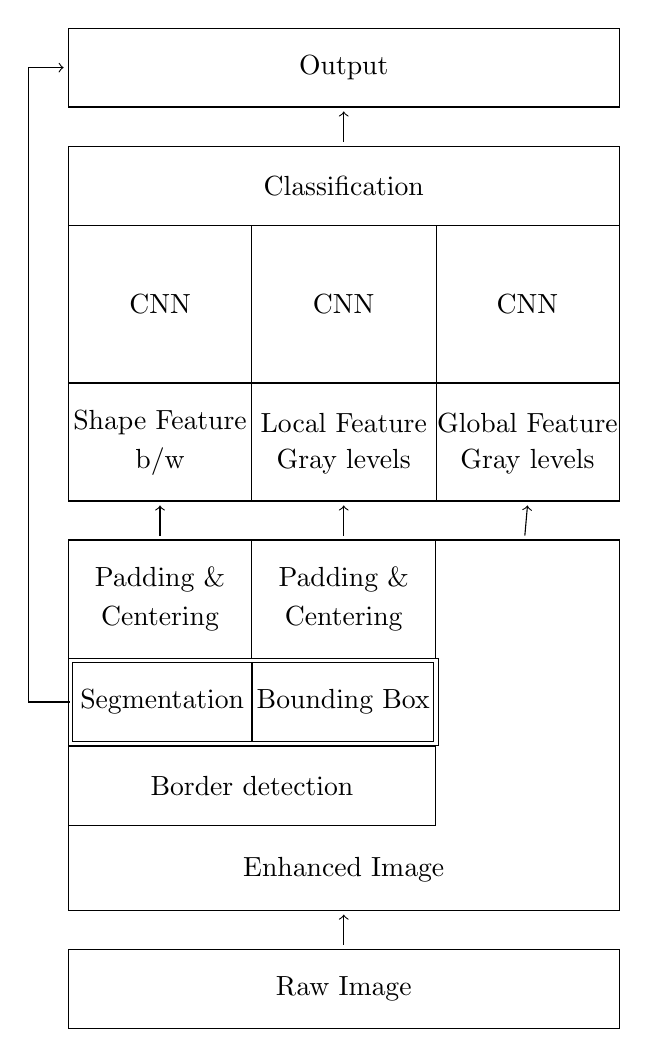
\begin{tikzpicture}

            % \draw[help lines] (0,0) grid (8.5,16);

            % Output
            \node[architecture_node_fullwidth,fill=waterblue,architecture_no_fill] (output) at (1,16) {Output};

            % Classificator
            % \node[architecture_box,minimum width=7.2cm,minimum height=4.7cm] (classification_architecture) at (.9,14.6) {};
            \node[architecture_node_fullwidth,fill=purple,architecture_no_fill] (classification) at (1,14.5) {Classification};
                    % CNN
                \matrix[architecture_node_nofill,minimum width=\onethird,minimum height=2cm,inner sep=0mm,fill=blue,architecture_no_fill] (cnn) at (1,13.5) {
                    \node {CNN}; & \node (cnn_local) {CNN}; & \node {CNN}; \\
                };
                \draw[black] (cnn_local.north east)--(cnn_local.south east);
                \draw[black] (cnn_local.north west)--(cnn_local.south west);

                    % INPUT
                \matrix[architecture_node_nofill,minimum width=\onethird,minimum height=1cm,inner sep=0mm,row sep=-0.51cm,fill=lightblue,architecture_no_fill] (cnn_features) at (1,11.5) {
                    \node (cnn_shape_feature) {Shape Feature}; & \node (cnn_local_feature) {Local Feature}; & \node (cnn_global_feature) {Global Feature}; \\
                    \node (cnn_shape_feature_color) {b/w}; & \node (cnn_local_feature_color) {Gray levels}; & \node (cnn_global_feature_color) {Gray levels}; \\
                };
                \draw[black] (cnn_local_feature.north east)--(cnn_local_feature_color.south east);
                \draw[black] (cnn_local_feature.north west)--(cnn_local_feature_color.south west);
            
            \draw[->] ($(classification.north) + (0,.05)$) -- ($(output.south) + (0,-0.05)$);

            % INPUT PREPROCESSING
                % Enhanced image
                \node[architecture_node_fullwidth,minimum height=4.7cm,fill=lightyellow,architecture_no_fill] (enhanced_image_box) at (1,9.5) {};
                \node[architecture_node_fullwidth,minimum height=1cm,anchor=south west,draw=none] (enhanced_image_label) at (1,4.8) {Enhanced Image};
                % \node[architecture_box,minimum width=7.2cm,minimum height=4.9cm] (preprocessing_architecture) at (.9,9.6) {};

                % Padding
                \matrix[architecture_node_nofill,minimum width=\onethird,minimum height=1cm,inner sep=0mm,row sep=-0.51cm,fill=lightred,architecture_no_fill] (cnn) at (1,9.5) {
                    \node (padding1) {Padding \&}; & \node (padding2) {Padding \&};\\
                    \node {Centering}; & \node (centering2) {Centering};\\
                };
                \draw[black] (padding2.north west)--(centering2.south west);

                % Segmentation & Bounding box
                \matrix[architecture_node_nofill,minimum width=\onethird - .6mm,minimum height=1cm,inner sep=.5mm,nodes={draw=black},fill=lightorange,architecture_no_fill,nodes={fill=orange,architecture_no_fill}] (segmentation_bounding_box) at (1,8) {
                    \node {Segmentation}; & \node {Bounding Box};\\
                };

                % Border detection & Region proposals
                \node[architecture_node_nofill,minimum width=2*\onethird,minimum height=1cm,fill=yellow,architecture_no_fill] (border) at (1,6.88) {Border detection};
            
            \draw[->] ($(segmentation_bounding_box.west) + (0.03,0)$) -- ($(segmentation_bounding_box.west) + (-0.5,0)$) -- ($(output.west) + (-0.5,0)$) -- ($(output.west) + (-0.05,0)$);
            \draw[->] ($(padding1.north) + (0,.05)$) -- ($(cnn_shape_feature_color.south) + (0,-0.05)$);
            \draw[->] ($(padding2.north) + (0,.05)$) -- ($(cnn_local_feature_color.south) + (0,-0.05)$);
            \draw[->] ($(enhanced_image_box.north) + (2.3cm,.05)$) -- ($(cnn_global_feature_color.south) + (0,-0.05)$);

            % Raw image
            \node[architecture_node_fullwidth,fill=green,architecture_no_fill] (rawim) at (1,4.3) {Raw Image};
            \draw[->] ($(rawim.north) + (0,.05)$) -- ($(enhanced_image_box.south) + (0,-0.05)$);

        \end{tikzpicture}
        \caption{Proposed defect detection system architecture}\label{fig:architecture}
    \end{figure}

    \par{
        The defect detection system architecture proposed in this paper is shown in figure \ref{fig:architecture}.
    }

    \par{
        Steel surfaces pictures of $1600\times 256$ pixels are taken at the input of the process. Since they may be taken under different light exposure conditions, some preprocessing is made to enhance the quality of the image, e.g. histogram equalization or linear scaling. Moreover, the images considered have three equal colours levels, therefore they are converted into gray levels, to save space. This first step is further described in \ref{section:image_preprocessing}.
    }
    \par{
        The aim of the architecture proposed in this paper is both to detect pixels representing steel imperfections and to classify those regions. Therefore, image segmentation is either obtained as an output of the system or it is needed in some step during the process. The latter situation can be achieved through a brute-force multi-scale sliding window, but to improve performances without reducing accuracy a particular implementation of a Region based CNN (R-CNN) \cite{ieee:7410526,ieee:7532516} is proposed in \ref{section:mc-cnn}. This R-CNN uses a MC-CNN to combine and to consider separately interesting regions, which are called proposals and which are described in \ref{section:region_proposals}.
    }
    \par{
        This reduces the computational cost of the system, compared with a naive sliding window.
    }
    \par{
        Moreover, both local and global information are combined to improve classification accuracy. This approach avoids the complexity of combining different scale information and handling windows with different classes of defects. A further description of this approach is provided in \ref{section:mc-cnn}, whereas in \ref{section:further-work} a challenger architecture is described, to compare the results of the proposed system with.
    }
    \par{
        One column of the MC-CNN is concerned with global information, and it is fed with the full enchanced image. Conceptually, this CNN learns to evaluate the probability of presence of the different types of defects in the whole surface picture. The other two columns consider local information instead. This local information is obtained from a further processing step, described in \ref{section:region_proposals}. Firstly, a contour detection algorithm (\ref{subsection:contour_detection}) is used to spot proposals. Secondly, image segmentation (\ref{subsection:segmentation}) is done, to feed the MC-CNN only with some interesting regions. This segmentation results in a black and white (b/w) map describing the shape of the plausible defects. One column of the MC-CNN is fed with this map, therefore it learns to classify regions only observing their border. The other column is fed with the portion of original image enveloped in the bounding box (\ref{subsection:bounding_box}) of the map, hence it is trained to consider luminance levels inside, outside and on the border of the considered proposals.
    }
    \par{
        Since defects may have different dimensions, the local information are centered in a $1600\times 256$ pixels black image.
    }
    \par{
        All the MC-CNN columns end with a softmax layer. However, they have different output size, as described in \ref{section:mc-cnn}. Their results are then combined in order to properly classify the local regions.
    }
    \par{
        Finally, if the classification outcome labels the region as defective, segmentation coordinates are kept. When all the proposals of the considered image have been processed, defective pixels of the same class are encoded together with RLE algorithm. If the surface is flawless, all this encodings are empty.
    }
    \section{Image preprocessing}
    Motivation and approach pith.
    
    \subsection{Compression, equalization and noise reduction}
        Explain need and method... cite articles that do the same, cite articles that introduce the methods \cite{Klette:2014:CCV:2584519}.

    \subsection{Edge detection filter}
        Cite main edge detection filters, explain approach (phase congruency) and previous use of wavelet in this field.. our approach and our evaluation of different wavelet families.
        \subsubsection{Phase congruency edge detection}
            Phase congruency.....  through wavelet .....
        \subsubsection{...}
            ..... Other steps .....
        \subsubsection{Maxima suppression}
            Describe maxima suppression....
        \subsubsection{Thresholding}
            Describe hysteresys thresholding....
            Table comparing different thresholding values....
        \subsubsection{Wavelet family}
            Present different wavelet families, euristic considerations, ....
            Table comparing different wavelet families....
        \subsubsection{Evaluation schema}
            Describe how we evaluated any choice.. optimization for example on confronting how much the defects area are highlighted.
            An effective approach to this black-box derivative-free global-optimization method is Bayesian Optimization \cite{rasmussen:williams:2006, arXiv:2018arXiv180702811F, arXiv:2012arXiv1206.2944S}
            Loss when we loose defects...
            Loss when we keep too much non defects area...
    \section{Detector}\label{section:region_proposals}
    \par{
        The second stage of the proposed architecture is the \emph{detector} of region proposals, which are then fed into the \emph{classificator} for classification, which is described in \emph{Section} \ref{section:mc-cnn}.
    }
    \par{
        The whole system relies on the \emph{detector} to spot one or more region of interest (ROI), which are the plausible candidates to be defective regions.
    }
    \par{
        To extract them, firstly an edge detector is used (\emph{Section \ref{subsection:contour_detection}}). Its output is a binary matrix describing the edges found. The alpha shape of this matrix is then used to segmentate ROIs (\emph{Section \ref{subsection:segmentation}}). Finally, the bounding box of the regions can be easily calculated (\emph{Section \ref{subsection:bounding_box}}).
    }
    \subsection{Edge detection}\label{subsection:contour_detection}
        \par{
            The first step towards segmentation consists of the detection of edges within the image. The usage of Kovesi algorithm (KA) \cite{mit:kovesiphase, googlescholar:kovesiphase} together with hysteretic edge follower \cite{Klette:2014:CCV:2584519}.
        }
        \par{
            KA is a \emph{phase congruency}-based edge detector. The main idea is that where the local frequency components of an image are in phase, there is an edge \cite{researchgate:morrone}. This concept is illustrated in \emph{Figure \ref{fig:phase-congruency}}.
        }
        \par{
            Some phase congruency metrics are based on Fourier analysis and on measuring the local energy \cite{researchgate:phase}, whereas KA exploits the log-Gabor wavelets. These are shown in \emph{Figure \ref{fig:gabor}}.
        }
    	\begin{figure}
    		\centering
    		\includegraphics[width=.9\linewidth]{graphics/architecture/phasecong}
    		\caption{Visualization of the phase congruency concept for a 1D signal. The sum (blue curve) of the frequency components (red and orange curves) gradually approaches a discontinuity where the components are in phase.}
    		\label{fig:phase-congruency}
    	\end{figure}
    	\begin{figure}
    		\centering
    		\includegraphics[width=\linewidth]{graphics/architecture/gabor}
    		\caption{Examples of log-Gabor wavelets with different directions and scales.}
    		\label{fig:gabor}
    	\end{figure}
		\par{
			Given a image and fixed a direction $u$, for each pixel $q$ a squared local window $W(q)$ is considered. It is an image crop centered in $q$. Then, $W(q)$ is convolved with the log-Gabor wavelets at different scales $n = 0 \dots N-1$, obtaining the complex number:
	    	\begin{equation*}
	    		z_{n} (q) = G_{n} * W(q) = r_{n} (q) e^{i \alpha_{n} (q)}.
	    	\end{equation*}
	    	Then, the phase congruency measure at $q$ is:
            \begin{equation*}
	            \mathcal{P} (q) = \frac{\max(0,\lvert \sum_{n} z_{n} (q) \rvert - T)}{\sum_{n} r_{n} (q) + \varepsilon},
            \end{equation*}
            where $T$ is a constant that soothes the effects of noise and $\varepsilon$ is a small value, used to avoid numerical problems concerning negligible values of $r_n$. 
        }
        \par{
            One of the advantages of this measure is that it is dimensionless. The concept behind this metric is illustrated in \emph{Figure \ref{fig:phase-congruency-metric}}.
        }
	    \begin{figure}
	    	\centering
	    	\includegraphics[width=\linewidth]{graphics/architecture/phasecong_metric}
	    	\caption{Phase congruency metric.}
	    	\label{fig:phase-congruency-metric}
	    \end{figure}
	    \par{
	    	The local window $W(q)$ size is $(2k+1)\times(2k+1)$, with $2k+1 \geq 3\lambda$.
		}
        \par{
        	$\mathcal{P}$ lies in the $[0,1]$ interval. However, as reported in \emph{Section \ref{section:results}}, the \emph{min-max normalization}
        	\begin{equation*}
        	\hat{\mathcal{P}}(q) = 255 \cdot \frac{\mathcal{P}(q)-\min_q\mathcal{P}(q)}{\max_q\mathcal{P}(q)-\min_q\mathcal{P}(q)}
        	\end{equation*}
        	 on KA output improves the performance of the detector stage.
        }
        \par{
        	KA is based on several parameters that need to be tuned to obtain an effective edge detector. In this paper, the \emph{number of scales} $N$, the \emph{number of orientations} $U$, the \emph{minimum wavelength} $\lambda$ and the \emph{scaling factor} $s$ of the wavelets are considered. Their tuning was performed through Bayesian optimization \cite{arXiv:2012arXiv1206.2944S,arXiv:2018arXiv180702811F, matlab:bayesian-opt}, as described in section \ref{subsection:segmentation}.
        }
        \par{
            It is not recommend to use directly the output of KA for image segmentation, since it is tipically susceptible to isolated edge-like patterns that arise in sparse locations within the image. Hence, a hysteretic edge follower was used to discard such patterns.
        }
        \par{
            Let $\mathcal{I}$ be the image, $\mathcal{Q} = \left\{q \in \mathcal{I} \colon \hat{\mathcal{P}}(q) > T_{high}\right\}$, $\Omega(q)$ the set of  pixels adjacent to $q$ and $\mathcal{E} = \empty$ the set of edge pixels.
        }
        \par{
            Then, the hysteretic edge follower calculates edge pixels as:
            \begin{enumerate}
    			\item $q_i \in \mathcal{Q};\; \mathcal{Q} = \mathcal{Q} \setminus \{q_i\};\;\mathcal{E} = \mathcal{E} \cup \{q_i\}$
    			\item $\forall q_j \in \Omega(q_i)$ if $\hat{\mathcal{P}}(q_j) > T_{low}$ then $\mathcal{E} = \mathcal{E} \cup \{q_j\}$ and repeat $(2)$ with $q_i = q_j$
    			\item if $\mathcal{Q} \neq \empty$ then repeat $(1)$
    		\end{enumerate}
        }
		\par{
			The final output is a binary matrix marking the positions of edge pixels. The hysteretic parameters \emph{low-threshold} $T_{low}$ and \emph{high-threshold} $T_{high}$ need to be properly tuned, in order to improve the effectiveness of edge detection, as illustrated in \emph{Figure \ref{fig:edge-detector-example}}. Therefore, they were free parameters during the Bayesian optimization, together with KA ones.
        }
    	\par{
    		The described techniques \texttt{MATLAB} implementation is freely available at \cite{kovesilibrary}.
    	}
    	\begin{figure} 		  
    		\includegraphics[width=\linewidth]{graphics/architecture/detector-ex}
    		\vskip .05cm
    		\includegraphics[width=\linewidth]{graphics/architecture/detector-ex-hysteresis-30-50}
    		\vskip .05cm \includegraphics[width=\linewidth]{graphics/architecture/detector-ex-hysteresis-60-100}
    		\vskip .05cm \includegraphics[width=\linewidth]{graphics/architecture/detector-ex-hysteresis-90-150}
    		\vskip .05cm
    		\caption{Output of the edge detector on a sample image using different thresholds $(T_{low},T_{high})$. Respectively, from top to bottom: $(30,50)$, $(60,100)$ and $(100,150)$. Standard parameters of the Kovesi algorithm has been used.}
    		\label{fig:edge-detector-example}
    	\end{figure}
    
    \subsection{Image Segmentation}\label{subsection:segmentation}
        \par{
            Given the plausible edges found by the previous step, image segmentation is performed banking on alpha shapes \cite{springer:10.1007/11907350_46}.
        }
        \par{
            The Delaunay triangulation $\mathcal{D}$ od a set of point $\mathcal{S}$ is the subset of all triangles $T = \left\{\left(a, b, c\right) \subset \mathcal{S}^3, a \neq b, b \neq c, a \neq c \right\}$ such that $t \in T, x \in \mathcal{S} \Rightarrow x \not\in \mathcal{C}\left(t\right)$, where $\mathcal{C}\left(t\right)$ is the circumcircle of $t$.
        }
        \par{
            The union of cells $c \in \mathcal{D}$ is called polytope of $\mathcal{D}$. 
            \begin{equation*}
                \mathcal{D}_\alpha = \left\{t \in T \colon r\left(\mathcal{C}\left(t\right)\right) < \alpha\right\},
            \end{equation*}
            where $r\left(\mathcal{C}\left(t\right)\right)$ is the radius of the circumcircle of $t$. The polytope of $\mathcal{D}_\alpha$ is called \emph{alpha-shape}.
        }
        \begin{figure}
            \centering
            \includegraphics[width=\linewidth]{graphics/architecture/detector-points}
            \includegraphics[width=\linewidth]{graphics/architecture/detector-a-shape}
            \includegraphics[width=\linewidth]{graphics/architecture/detector-a-shape-better-radius}
            \caption{Alpha shape with different alphas of a set of points.}\label{fig:example-alpha-shape}
        \end{figure}
        \begin{figure}
            \centering
            \includegraphics[width=\linewidth]{graphics/architecture/detector-convhull}
            \caption{Convex hull of a set of points.}\label{fig:example-convex-hull}
        \end{figure}
        \par{
            As an example, in \emph{Figure \ref{fig:example-alpha-shape}} are compared the alpha-shapes with different $\alpha$ values of a set of points. In \emph{Figure \ref{fig:example-convex-hull}} is shown the convex-hull of the same set of points. The choice of alpha shapes for the given task is clear.
        }
        \par{
            However, in order to obtain topologically correct image segmentation, three parameters need to be properly chosen \cite{springer:10.1007/11907350_46}. These are the \emph{alpha-radius} $\alpha$, the \emph{hole-thresholding} $T_{hole}$ and the \emph{region-thresholding} $T_{region}$ \cite{matlab:alpha-shape}.
        }
        \par{
            The first is the value of $\alpha$, the second is the maximum area of interior holes that is filled and the third is the largest area that is suppressed (ignored).
        }
        \par{
            Observe that the latter is useful to soothe the effects of noisy edge detections.
        }
        \par{
            However, tuning them manually is quixotic, hence they are choosen through Bayesian optimization.
        }
        \par{
            The segmentation step outputs a set of pixels, which can be compared with the ideal segmentation, i.e. only the pixels within some defective region.
        }
        \par{
            Therefore, the goodness of fit of the set of proposed pixels $\left(X\right)$ to the ideal pixels $\left(Y\right)$ can be measured as:
            \begin{equation*}
                \chi\left(X, Y\right) = \frac{2 \lvert X \cap Y \rvert}{\lvert X \rvert + \lvert Y \rvert}.
            \end{equation*}
        }
        \par{
            Hence, the loss function is:
            \begin{equation*}
                \mathcal{L}\left(X, Y\right) = 1 - \chi\left(X, Y\right).
            \end{equation*}
        }
	    \par{
		    DESCRIVERE ACCURATEZZA
		    \begin{equation*}
		    \mathcal{A}\left(X, Y\right) = \frac{\lvert X \cap Y \rvert}{\lvert Y \rvert}
		    \end{equation*}
		}
        \par{
            The acquisition function used is \emph{expected-improvement-plus} \cite{matlab:acquisition}.
        }
        \par{
            As a final consideration, using alpha shape lessen the detrimental effect of the noise in edge detection. Indeed, outliers are suppressed by the hole threshold and region threshold parameteres.
        }
        \par{
            The regions of this alpha shape are the ROIs, which are fed into the \emph{classificator}.
        }
    \subsection{Bounding box}\label{subsection:bounding_box}
        \par{
            The bounding box of a ROI can be easily calculated considering the extremal coordinates of its pixels.
        }
        \par{
            Let \texttt{pixels} be the $M \times 2$ matrix of the coordinates of the pixels within the ROI, with $M$ the number of pixels. Then the bounding box is: 
        }
        \par{
            \begin{BVerbatim}

                 _         _         
                | minX minY |
bounding_box =  | maxX maxY |
                 -         - 
            \end{BVerbatim}
        }
        \par{
            Where:
        }
        \par{
            \begin{BVerbatim} 

        minX = min(pixels(:,1))
        maxX = max(pixels(:,1))
        minY = min(pixels(:,2))
        maxY = max(pixels(:,2))
   
            \end{BVerbatim}
        }
        \par{
            As a first approximation, the implementation of the detector was done to output the bounding boxes instead of the alpha shape. Therefore, the $X$ set in \emph{Section \ref{subsection:segmentation}} is characterized by all the pixels inside the bounding box of the alpha shape regions.
        }

    \section{Classificator}\label{section:mc-cnn}
    \par{
        The ROIs are then fed into the third part of the proposed architecture, the \emph{classificator}, and properly classified as flawless or flawed; in the latter case, they are assigned a defect class.
    }
    \begin{figure}
        \centering
        \begin{tikzpicture}
            % image
            \node[circle, draw] (input) at (0,0) {I};
    
            % preprocessed image
            \node[rectangle, draw] (p1) at ($(input) + (1.5,2)$) {P};
            \node[rectangle, draw] (p2) at ($(input) + (1.5,.5)$) {P};
            \node (p3) at ($(input) + (1.5,-.5)$) {\vdots};
            \node[rectangle, draw] (p4) at ($(input) + (1.5,-2)$) {P};
    
            % image to preprocessed image
            \draw[->] ($(input) + (0.5, 0)$) -- ($(p1) + (-0.3, 0)$);
            \draw[->] ($(input) + (0.5, 0)$) -- ($(p2) + (-0.3, 0)$);
            \draw[->] ($(input) + (0.5, 0)$) -- ($(p4) + (-0.3, 0)$);
    
            % cnn
            \node[rounded rectangle, draw, minimum width=2.5cm, minimum height=1cm] (cnn1) at ($(p1) + (2,0)$) {CNN};
            \node[rounded rectangle, draw, minimum width=2.5cm, minimum height=1cm] (cnn2) at ($(p2) + (2,0)$) {CNN};
            \node[minimum width=2.5cm, minimum height=1cm] (cnn3) at ($(p3) + (2,0)$) {\vdots};
            \node[rounded rectangle, draw, minimum width=2.5cm, minimum height=1cm] (cnn4) at ($(p4) + (2,0)$) {CNN};
    
            % preprocessed to cnn
            \draw[->] ($(p1) + (0.5, 0)$) -- ($(cnn1) + (-1.2, 0)$);
            \draw[->] ($(p2) + (0.5, 0)$) -- ($(cnn2) + (-1.2, 0)$);
            \draw[->] ($(p4) + (0.5, 0)$) -- ($(cnn4) + (-1.2, 0)$);
    
            % classifier
            \node[rounded rectangle, draw] (classifier) at ($(cnn3) + (2.5,0.5)$) {NN};
    
            % cnn to classifier
            \draw[->] ($(cnn1) + (1.3, 0)$) -- ($(classifier) + (-.5, .2)$);
            \draw[->] ($(cnn2) + (1.3, 0)$) -- ($(classifier) + (-.5, 0)$);
            \draw[->] ($(cnn4) + (1.3, 0)$) -- ($(classifier) + (-.5, -.2)$);
    
            % output
            \node[circle, draw] (output) at ($(classifier) + (1.3,0)$) {O};
    
            % classifier to output
            \draw[->] ($(classifier) + (.5, 0)$) -- ($(output) + (-.45, 0)$);
    
        \end{tikzpicture}
        \caption{General structure of a MC-CNN}\label{fig:mc-cnn}
    \end{figure}
    \par{
        The \emph{classificator} is structured as a MC-CNN, which in general has the structure illustrated in figure \ref{fig:mc-cnn}. 
    }
    \par{
        Firstly, the input image I is preprocessed to extract $n$ column input P.
    }
    \par{
        Secondly, these P are fed into different CNNs in parallel, therefore all the columns are independent one another. 
    }
    \par{
        Finally, the output of the MC-CNN columns is combined through a classificator, e.g. a neural network (NN), to produce the final output.
    }
    \par{
        The choice of using a MC-CNN is due to several reasons, beyond the proved effectiveness described in \cite{ieee:6248110}.
    }
    \par{
        Primarily, the training of a MC-CNN is highly parallelizable, indeed the different columns can learn separately one from another, once their correspective input is prepared.
    }
    \par{
        Moreover, it is possible to merge both local and global information in a far easier way then using a traditional, single-column, CNN. Indeed, instead of focusing only on a rectangular area, which brings only the local information about the plausible defect, with a MC-CNN it is immediate to add another column concerned with the whole image.
    }
    \par{
        This is the main point in favour of MC-CNN, since the class of a defect may be inferred using global patterns, such as the number of similar area. Imagine, for example, an error burst on the surface. Although traditional single-column CNNs may consider directly the input to the global column, this would face problems regarding the presence of multiple defects classes on the same surface. Therefore, a MC-CNN approach with some columns concerning local information and other focusing on global patterns is heuristically better.
    }
    \par{
        In \ref{section:further-work} another approach to combine such information through a CNN is described. Although possible, is patently more convoluted then the MC-CNN approach. It would still be interesting to compare them in order to better evaluate the effectiveness of the proposed architecture. 
    }
    \par{
        Observe that the output of global column must be calculated only once per each image, since it is constant throughtout the single surface, hence both the training and the predicting process can be lighten.
    }
    \par{
        Finally, as an incidental outcome, it is possible to further study the amount of contribution of the different columns in accurately determining the defective class, if any, of the considered area. This considerations are reported in \ref{section:results}.
    }
    \par{
        The proposed MC-CNN has three columns, namely a \emph{shape}, a \emph{local} and a \emph{global} column.
    }
    \par{
        A final consideration about the architecture training has to be done in order to comprehend the upper bound reported in \ref{section:results}. Indeed, the \emph{classificator} has been implemented before the \emph{detector}. In fact, although the former relies on the latter for the ROIs and their relative features (described in \ref{section:shape-column}, \ref{section:local-column} and \ref{section:global-column}), it has been preempting supposed to have an ideal \emph{detector}, i.e. one which proposes the optimal ROIs.
    }
    \par{
        This effort-outcome oriented approach has been done for two main reasons.
    }
    \par{
        Firstly, it highlights the upper bound reachable with the whole architecture.
    }
    \par{
        Secondly, dividing the \emph{detector} outcome from the \emph{classificator} input during the training allows to export the trained MC-CNN and to use it within the challenger architecture, explained in \ref{section:challenger}.
    }
    \subsection{Shape column}\label{section:shape-column}
        \par{
            The \emph{shape column} is concerned to learn from the shape of the proposed region. This is fed into the CNN as a binary matrix, in which ones represent points in the border of the area.
        }
        \begin{figure}
            \centering
            \includegraphics[width=\linewidth]{graphics/architecture/mc-cnn-shape}
            \caption{Shape column input.}\label{fig:mc-cnn:shape-input}
        \end{figure}
        \par{
            An example of this binary images is given in figure \ref{fig:mc-cnn:shape-input}. The shape is centered in a $1600\times 256$ black image. Indeed, the size of the input is set to the largest area that could be found, i.e. a defect spanning over the entire surface. The shape is centered to ensure that the classificator is translation independent. 
        }
        \par{
            ** EXPLAIN WHY NO FAKE REGIONS **
        }
        \begin{figure}
            \centering
            % \includegraphics[]{}
            \caption{Shape column CNN layers}\label{fig:mc-cnn:shape-structure}
        \end{figure}
        \par{
            The layers of this CNN are shown in \ref{fig:mc-cnn:shape-structure}. *** ... explanation, dimensioning, type of layers .... Stats on defects shapes.... ***
        }
        \par{
            The output layer is a $n$-dimensional vector, where $n$ is the number of defect classes. Each entry of this vector describe the confidence of the network in considering the input shape as related to one of the $n$ defect classes.
        }
    \subsection{Local column}\label{section:local-column}
        \par{
            The \emph{local column} is thought to consider luminance levels around the border of the defect, to learn from the local context ** NO FAKE; ONLY CLASS **.
        }
        \begin{figure}
            \centering
            \includegraphics[width=\linewidth]{graphics/architecture/mc-cnn-local}
            \caption{Local column input.}\label{fig:mc-cnn:local-input}
        \end{figure}
        \par{
            Therefore, the column is fed with the grey scale portion of the image inside the bounding box of the considered region. As an example, in figure \ref{fig:mc-cnn:local-input} is illustrated a plausible input to the \emph{local column}.
        }
        \par{
            This grey scale portion is generated from the shape of the region and the original image.
        }
        \par{
            Firstly, the bounding box of the shape is calculated. Secondly, the original image outside the bounding box is discarded. Finally, the cropped image is centered in a black $1600\times 256$ picture. The reasons behind the centering and the dimensioning of the input are the same described in \ref{section:shape-column}.
        }
        \begin{figure}
            \centering
            % \includegraphics[]{}
            \caption{Local column CNN layers}\label{fig:mc-cnn:local-structure}
        \end{figure}
        \par{
            The layers of this CNN are shown in \ref{fig:mc-cnn:local-structure}. *** ... explanation .... Stats on defects shapes.... ***
        }
        \par{
            The output layer is analogous to the one in \ref{section:shape-column}.
        }
    \subsection{Global column}\label{section:global-column}
        \begin{figure}
            \centering
            \includegraphics[width=\linewidth]{graphics/architecture/mc-cnn-global}
            \caption{Global column input.}\label{fig:mc-cnn:global-input}
        \end{figure}
        \par{
            The \emph{global column} is concerned in detecting global patterns, like zipper cracks. Hence, it is fed with the whole image. An example of input is shown in figure \ref{fig:mc-cnn:global-input}. The importance of this column is clear from the observations made in \ref{subsection:defects}. Indeed, when two different classes are locally equal, the global column is determinant to correctly classify the defects.
        }
        \begin{figure}
            \centering
            % \includegraphics[]{}
            \caption{Global column CNN layers}\label{fig:mc-cnn:global-structure}
        \end{figure}
        \par{
            *** structure, explanation, output ***\\
            *** MAYBE OUTPUT AS MULTIPLE COMBINATIONS CLASSES? *** \\
            *** DESCRIBE STRUCTURE, RATIONALE BEHIND DIMENSIONING, USE DEFECT STATS ***
        }
    \subsection{Final classifier}
        \par{
            The outcomes of the different columns of a MC-CNN are then combined to obtain the final output. In the proposed architecture, this combination is done through a neural network, since a manual tuning of such combination would be ineffective. Moreover, this is used to establish thresholding.
        }
        \begin{figure}
            \centering
            \begin{tikzpicture}
                % input layer
                \foreach \i in {0,...,11} % TODO fix
                    \node[circle, draw, minimum height=1, minimum width=1,fill=blue] (input \i) at (0,-\i*0.5) {};

                % hidden layer
                \foreach \i in {0,...,7} % TODO fix
                    \node[circle, draw, minimum height=1, minimum width=1,fill=orange] (hidden \i) at ($(input 2) + (2,-\i*0.5)$) {};

                % from input to hidden layer
                \foreach \i in {0,...,11}
                    \foreach \j in {0,...,7}
                        \draw ($(input \i) + (.2,0)$) -- ($(hidden \j) + (-.2,0)$);

                % output layer
                \foreach \i in {0,...,4} % TODO fix
                    \node[circle, draw, minimum height=1, minimum width=1,fill=yellow] (output \i) at ($(hidden 1) + (2,-\i*0.5)$) {};

                % from hidden to output layer
                \foreach \i in {0,...,7}
                    \foreach \j in {0,...,4}
                        \draw ($(hidden \i) + (.2,0)$) -- ($(output \j) + (-.2,0)$);

                % from output to softmax layer
                \foreach \i in {0,...,4}
                    \draw ($(output \i) + (.2,0)$) -- ($(output \i) + (2,0)$);

                % softmax layer
                \node[rounded rectangle, fill=white, minimum width=3cm,draw,rotate=-90] (softmax) at ($(output 2) + (1,0)$) {Softmax};

                % legend
                \node[rectangle, draw, fill=yellow, minimum width=1, minimum height=1] (output label color) at ($(output 0) + (0,1)$) {};
                \node[anchor=west] (output label) at ($(output label color) + (.2,0)$) {Output layer};

                \node[rectangle, draw, fill=orange, minimum width=1, minimum height=1] (hidden label color) at ($(output label color) + (0,.5)$) {};
                \node[anchor=west] (hidden label) at ($(hidden label color) + (.2,0)$) {Hidden layer};

                \node[rectangle, draw, fill=blue, minimum width=1, minimum height=1] (input label color) at ($(hidden label color) + (0,.5)$) {};
                \node[anchor=west] (input label) at ($(input label color) + (.2,0)$) {Input layer};

                \node[anchor=west] (legend label) at ($(input label color) + (-.25,.5)$) {\underline{Legend}};
            \end{tikzpicture}
            \caption{Final classifier structure.}\label{fig:mc-cnn:final-classifier-structure}
        \end{figure}
        \par{
            In figure \ref{fig:mc-cnn:final-classifier-structure} the structure of the last layer of the architecture is shown.
        }
        \par{
            The first layer is constrained to the output size of the three columns, i.e. *** TODO COMPLETARE... *** Then there is an hidden layers with $7$ activation units, and finally the output layer with $5$ neurons. The output is passed through a softmax layer, hence the final output describe the confidence per each class.
        }
        \par{
            Observe that bias units have not been included in the picture.
        }
        \par{
            ** DISPLAY WEIGHTS, infer what matters most to determine output **
        }
        \par{
            The results of this architecture are shown in \ref{section:results}.
        }

    \section{Results}\label{section:results}
    Review the article, make some considerations on results
    Observe that this architecture is dealing with different sixze image, interesting.....!!!

    \subsection{Detector}
        \par{
		    ***DESCRIVERE ACCURATEZZA***
		    \begin{equation*}
		    \mathcal{A}\left(X, Y\right) = \frac{\lvert X \cap Y \rvert}{\lvert Y \rvert}
		    \end{equation*}
		}
        \begin{figure}
    	\centering
    	\includegraphics[width=\linewidth]{graphics/results/segmentation_opt_class1}
    	\caption{Bayesian optimization of class 1 detector}\label{fig:bayesopt-class1}
    \end{figure}
    \begin{figure}
    	\centering
    	\includegraphics[width=\linewidth]{graphics/results/segmentation_opt_class1}
    	\caption{Bayesian optimization of class 2 detector}\label{fig:bayesopt-class2}
    \end{figure}
    \begin{figure}
    	\centering
    	\includegraphics[width=\linewidth]{graphics/results/segmentation_opt_class3}
    	\caption{Bayesian optimization of class 3 detector}\label{fig:bayesopt-class3}
    \end{figure}
    \begin{figure}
    	\centering
    	\includegraphics[width=\linewidth]{graphics/results/segmentation_opt_class4}
    	\caption{Bayesian optimization of class 4 detector}\label{fig:bayesopt-class4}
    \end{figure}
    \begin{table}
		\centering
		\begin{tabular}{|c|c|c|c|c|}
			\hline
			\textbf{Parameters} & \textbf{Class 1} & \textbf{Class 2} & \textbf{Class 3} & \textbf{Class 4}\\ \hline
			$N$ & 3 & 4 & 5 & 4 \\ \hline
			$U$ & 15 & 7 & 5 & 15 \\ \hline
			$\lambda$ & 3.9199 & 2.3621 & 4.9810 & 3.5076 \\ \hline
			$s$ & 2.1161 & 1.5552 & 1.5559 & 1.4307 \\ \hline
			$T_{low}$ & 59 & 77 & 60 & 59 \\ \hline
			$T_{high}$ & 113 & 212 & 104 & 179 \\ \hline
			$\alpha$ & 7 & 8 & 6 & 6 \\ \hline
			$T_{hole}$ & 9593 & 6460 & 7179 & 9986 \\ \hline
			$T_{region}$ & 510 & 942 & 727 & 1134 \\ \hline
		\end{tabular}
		\vspace{0.25cm}
		\caption{Optimal parameters obtained for each class detector with Bayesian optimization.}\label{table:bayesopt-params}
	\end{table}
	\begin{figure}
		\centering
		\includegraphics[width=\linewidth]{graphics/results/acc-segmentation-class1}
		\vskip .05cm
		\includegraphics[width=\linewidth]{graphics/results/acc-segmentation-class2}
		\vskip .05cm
		\includegraphics[width=\linewidth]{graphics/results/acc-segmentation-class3}
		\vskip .05cm
		\includegraphics[width=\linewidth]{graphics/results/acc-segmentation-class4}
		\vskip .05cm
		\caption{INSERIRE}\label{fig:segmentation-test}
	\end{figure}
	\begin{table}
		\centering
		\begin{tabular}{|c|c|c|c|c|c|}
			\hline
			\textbf{Detector} & \textbf{Eq.} & \textbf{MinMax} & \textbf{Batch size} & \textbf{Loss} & \textbf{Accuracy}\\ \hline
			1 & yes & no & 5 & 4 & 4 \\ \hline
			2 & no & yes & 5 & 15 & 4\\ \hline
			3 & yes & yes & 4.9810 & 3.5076 & 4\\ \hline
		\end{tabular}
		\vspace{0.25cm}
		\caption{Optimal parameters obtained for each class detector with Bayesian optimization.}\label{table:bayesopt-params}
	\end{table}
	\begin{figure}
		\centering
		\includegraphics[width=\linewidth]{graphics/results/detector-result-class1}
		\vskip .05cm
		\includegraphics[width=\linewidth]{graphics/results/detector-result-class1-edges}
		\vskip .05cm
		\includegraphics[width=\linewidth]{graphics/results/detector-result-class1-segmentation}
		\vskip .05cm
		\includegraphics[width=\linewidth]{graphics/results/detector-result-class1-bounding-box}
		\vskip .05cm
		\caption{INSERIRE}\label{fig:detector-results-1}
	\end{figure}
	\begin{figure}
		\centering
		\includegraphics[width=\linewidth]{graphics/results/detector-result-class2}
		\vskip .05cm
		\includegraphics[width=\linewidth]{graphics/results/detector-result-class2-edges}
		\vskip .05cm
		\includegraphics[width=\linewidth]{graphics/results/detector-result-class2-segmentation}
		\vskip .05cm
		\includegraphics[width=\linewidth]{graphics/results/detector-result-class2-bounding-box}
		\vskip .05cm
		\caption{INSERIRE}\label{fig:detector-results-2}
	\end{figure}
	\begin{figure}
		\centering
		\includegraphics[width=\linewidth]{graphics/results/detector-result-class3}
		\vskip .05cm
		\includegraphics[width=\linewidth]{graphics/results/detector-result-class3-edges}
		\vskip .05cm
		\includegraphics[width=\linewidth]{graphics/results/detector-result-class3-segmentation}
		\vskip .05cm
		\includegraphics[width=\linewidth]{graphics/results/detector-result-class3-bounding-box}
		\vskip .05cm
		\caption{INSERIRE}\label{fig:detector-results-3}
	\end{figure}
	\begin{figure}
		\centering
		\includegraphics[width=\linewidth]{graphics/results/detector-result-class4}
		\vskip .05cm
		\includegraphics[width=\linewidth]{graphics/results/detector-result-class4-edges}
		\vskip .05cm
		\includegraphics[width=\linewidth]{graphics/results/detector-result-class4-segmentation}
		\vskip .05cm
		\includegraphics[width=\linewidth]{graphics/results/detector-result-class4-bounding-box}
		\vskip .05cm
		\caption{INSERIRE}\label{fig:detector-results-4}
	\end{figure}

    \subsection{Classificator}
    \par{

    }
    \begin{figure}
        \centering
        % \includegraphics[width=.8\linewidth]{graphics/results/mc-cnn-local-confusion}
        \caption{Local column confusion matrix on ideal input.}\label{fig:local-confusion}
    \end{figure}
    \begin{table}
        \centering
        \normalsize
        \caption{Local column comparisons}\label{table:results:local-comparisons}
    \end{table}
    \par{
        ** COMPARISONS with / without equalization local column **
    }
    \par{
        ** COMPARISONS crop / spreader local column **
    }
    \subsection{Architecture implementation}
    \par{
        The whole system implementation can be found in the \href{https://github.com/antonioterpin/wavelet_ml}{\texttt{GitHub}} repository \cite{antonioterpin:github}.
    }

\section{Further work}\label{section:further-work}
    \par{
        This work can be further developed in many ways.
    }
    \subsection{Proposed architecture improvement}
    \par{
        Firstly, it would be interest to implement and train the shape column, preeptively discarding misleading data, and the global column and measure their contribution. The structure of the shape column may be identical to the local column, described in \emph{Section \ref{section:local-column}}.
    }
    \par{
        Regarding the local column, some padding could be considered around defective regions, to fed the CNN also with some more pixels outside the border.
    }
    \par{
        Secondly, the final classifier should be implemented to realize the end-to-end system and evaluate its performance.
    }
    \par{
        Thirdly, as announced in \emph{Section \ref{section:local-column}}, both the local and the shape column could be fed with a cropped image. One could attempt to preemptively discard these outliers and try to optimize the other samples with a smaller input and, hence, more traditional classificators.
    }
    \begin{table*}
        \centering
        \normalsize
        \begin{tabular}{|c|c|c|c|c|c|}
            \hline
            \textbf{Cropping size} & \textbf{Class No.1 outliers} & \textbf{Class No.2 outliers}& \textbf{Class No.3 outliers} & \textbf{Class No.4 outliers} & \textbf{Overall outliers}\\\hline
            $800\times 800$ & $0\%$ & $0\%$ & $1.47\%$ & $1.06\%$ & $0.88\%$\\
            $512\times 512$ & $0\%$ & $0\%$ & $2.94\%$ & $3.99\%$ & $2.11\%$\\
            $256\times 256$ & $0\%$ & $0\%$ & $6.61\%$ & $17.57\%$& $6.42\%$\\
            \hline
        \end{tabular}
        \vspace{0.5cm}
        \caption{Cropping examples.}\label{table:cropping}
    \end{table*}
    \par{
        Some examples of interesting cropping size are shown in \emph{Table \ref{table:cropping}}.
    }
    \subsection{Challenger}
    \par{
        Some comparisons with a challenger architecture are needed to evaluate the effectiveness of the proposed system.
    }
    \par{
        As an example, a well-known \emph{sliding window} classificator could be used.
    }
    \subsubsection{Sliding window architecture}
        \par{
            The idea behind this architecture is to crop the input image at different locations (eventually all the ones possible, as in this paper) and use a classifier to assign to the pixels of the considered region an array of confidences.
        }
        \begin{figure}
            \centering
            \begin{tikzpicture}
                % Image
                \node[rectangle, draw, minimum width=3cm, minimum height=3cm] (image) at (0,0) {Image};
                % Window
                \node[rectangle, draw=red, minimum width=.8cm, minimum height=.8cm] (window) at ($(image) + (.3,.9)$) {};
                % Sliding window
                \draw[->, draw=red] ($(window) + (.2,0)$) -- ($(window) + (1,0)$);
                \draw[->, draw=red] ($(window) + (0,-.2)$) -- ($(window) + (0,-.7)$);
                % Classifier
                \node[rounded rectangle, draw, minimum width=2cm, minimum height=1cm] (classifier) at ($(image) + (2.5,0)$) {Classifier};
                \draw[->,draw=blue] ($(window) + (0,0)$) -- (classifier);
                % Confidence map
                \node[rectangle,draw,minimum width=3cm, minimum height=3cm] (confidence map) at ($(classifier) + (2.5,0)$) {Confidence map};
                \node[rectangle, draw=red, minimum width=.8cm, minimum height=.8cm] (confidence map window) at ($(confidence map) + (.3,.9)$) {};
                \draw[->, draw=red] ($(confidence map window) + (.2,0)$) -- ($(confidence map window) + (1,0)$);
                \draw[->, draw=red] ($(confidence map window) + (0,-.2)$) -- ($(confidence map window) + (0,-.7)$);
                \draw[->,draw=blue] (classifier) -- ($(confidence map window)$);
            \end{tikzpicture}
            \caption{Sliding window architecture}\label{fig:sliding-window}
        \end{figure}
        \par{
            This cropped regions may overlap. In those circumstances, an heuristic to combine different values of confidences is needed.
        }
        \par{
            In \emph{Figure \ref{fig:sliding-window}} the sketch of this architecture is shown. In the illustration the resulting map, called \emph{confidence map}, is associated to an array of confidences relative to the possible labels. 
        }
        \par{
            The \emph{confidence map} is then used along with some image segmentation tecnique to spot defective regions. In particular, a $n+1$ levels whatershed algorithm is proposed in \emph{Section \ref{section:challenger:image-segmentation}}.
        }
        \par{
            Since defects may have different dimensions, more refined tecniques could be used to improve the accuracy of the challenger. However, these are outside the scope of this work, and they are proposed as a further development in \emph{Section \ref{section:further-work}}. Moreover, the segmentation tecnique proposed in \emph{Section \ref{section:challenger:image-segmentation}} soothes this problem, since it combines local information from different areas to build the defective regions.
        }
    \subsubsection{Image segmentation}\label{section:challenger:image-segmentation}
        \par{
            The \emph{confidence map} is used to segmentate the image through a $n+1$ levels whatershed algorithm. However, since the defective regions are always disjunct, the problem can be reduced to a binary whatershed algorithm \cite{ieee:87344} considering all the defective classes as one, and distinguishing them only later. The $n+1$ levels whatershed algorithm is left as a further development in \emph{Section \ref{section:further-work}}.
        }
        \par{
            As a final remark about the challenger, it is patent that even this naive implementation is far more involved then the proposed architecture, and the reason lies on the image segmentation approach.
        }
    \par{
        Moreover, the challenger could be further refined. As an example, a multi-scale approach could be considered, since the challenger does not take into account the variability of defects dimensions. To solve this flaw, \emph{image pyramids} could be used.
    }
    \par{
        Finally, an interesting development would be to investigate further a segmentation with overlapping (adjacent) regions, when there are more classes then foreground/background only. Towards this multi-level segmentation, it would be interesting to consider a non-binary whatershed-based algorithm.
    }
    % \section*{Acknowledgment}
    The authors would like to thank...
    
    \bibliographystyle{IEEEtran}
    \bibliography{references}

\end{document}

